\clearpage
\section{Model Estimation and Selection}\label{app:b}\label{app:g}
This appendix records feature selection, fitting conventions and research chronology for the strategy-specific sizing policies and the capital allocator.

\subsection{Feature and Model Selection}\label{app:feature-selection}\label{sec:10}

Section~\ref{app:features} lists the 27 retained put inputs and their availability conventions. Future trade profits serve as training outcomes, never current inputs.


\subsubsection*{Variance Premium Features}

One additional block compares squared IV with forecast annualized variance. Its forecast uses exponentially weighted squared daily returns, with a 20-session half-life and at least 63 observations. Multiplication by 252 annualizes the estimate. The block adds the spread, a historical z-score and forecast-to-implied variance ratio, with availability flags.


\begin{equation*}\text{Variance spread}=IV^2-\widehat{\sigma}_{\rm RV}^{\,2}.\end{equation*}

IV and forecast volatility enter in decimal units, so the spread is a variance difference. Downside-put skew prevents interpreting it as a clean underlying variance-risk-premium estimate. The EWMA block is a tested addition; it is not part of the retained 27-input put baseline.


\begin{figure}[H]\centering
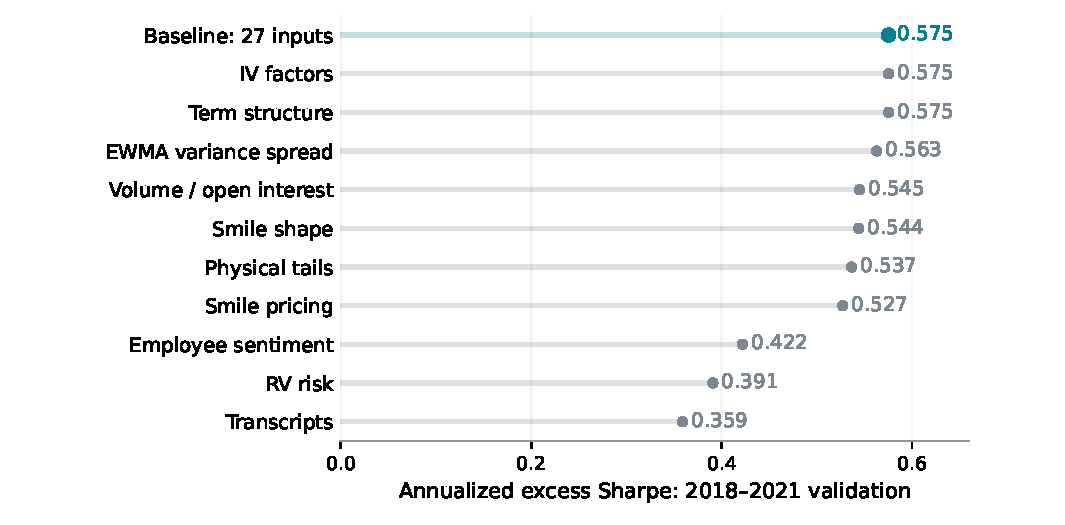
\includegraphics[width=\linewidth]{feature_validation.pdf}
\caption{Original feature exploration at the 18-month baseline. Scores use 2018--2021 validation and the archived \$345 million research account; funded policy comparisons use \$10 million. The three highest scores tie exactly.}\label{fig:feature-validation}
\end{figure}

We rank 33 archived screened configurations by 2018--2021 validation excess Sharpe within the established 30-day, 25-delta design. Feature, window and action-menu experiments form this grid. Baseline, IV-factor and term-structure scores tie exactly at 0.575; alphabetical configuration ordering retains the baseline. The selected specification has 27 inputs, an 18-month window and 50/75/100\% sizes.


Archived selection scores use a \$345 million research account; funded replays use \$10 million. This split selects the sizing procedure within the established contract design and pair roster. Section~\ref{app:research-chronology} records extension selection histories.


\FloatBarrier

\subsection{Monthly Refitting Timeline}\label{app:refitting-timeline}

\begin{figure}[!htbp]\centering
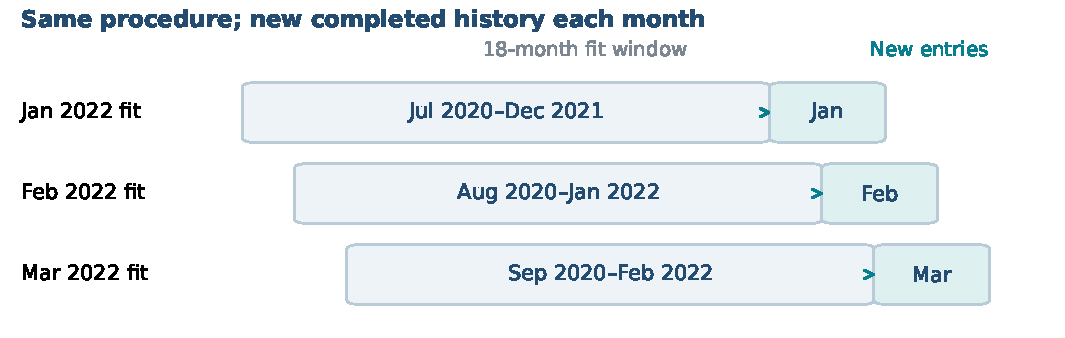
\includegraphics[width=\linewidth]{refit_timeline.pdf}
\caption{Monthly put-policy refitting. Only completed outcomes whose signal dates fall in the displayed 18-month window enter each fit. The selected model settings remain fixed; the tree and size assignments update.}\label{fig:refit-timeline}
\end{figure}


\FloatBarrier

\subsection{Entry Policy Optimization}\label{app:entry-optimization}

Put entry sizing follows Section~\ref{sec:11}. CEM uses 50 rounds of 192 maps, 19 elites and seed 2026. Probabilities start uniform; updates mix 30\% prior probability and 70\% elite frequency, shrink by 0.97 and add 0.03 uniformly. Constant maps and the incumbent are anchors. Separate rounded-contract paths supply daily training profits; funded NAV returns supply evaluation Sharpe. Put memory and training labels retain a \$0.65 option commission; funded evaluation uses \$0.03 for every policy.


The straddle ridge fit uses median centers, standard deviations floored at 0.001, clipped inputs within \(\pm\)5, penalty 100 with no intercept penalty, and equal total weight per date. Full-size completed profit is its target. Score terciles define contexts; all 27 size maps are evaluated on aggregate daily paths. Ties favor lower exposure. The 60-month window requires 128 examples. Only 4,116 training rewards are finite; the policy still handles all 35,774 proposals.



\subsection{Q-Function Specification and Convergence}\label{app:q-convergence}


The Q-function basis, state normalization, ridge penalties and weekly regression weighting are specified in Section~\ref{sec:allocation}. All 81 monthly fits were checked at 200, 500, 1,000 and 2,000 updates. Later actions are identical across budgets for the four reported \(\lambda\) values.



\FloatBarrier
\subsection{Research Chronology and Statistical Inference}\label{app:research-chronology}
Every fit uses strictly completed past outcomes. Put selection ranks 33 archived screened configurations by 2018--2021 scores before the \$10 million replay. The straddle's 48- and 60-month windows tie at validation Sharpe 0.775; later Sharpes of 0.960 and 1.041 informed refinement. The four displayed Q preferences illustrate researched risk choices, not a single validation-winning policy. The original selection and full results remain in \path{reports/signal_allocation_discount}. The put-sizing gain is 0.208, with a paired 95\% interval of -0.103 to +0.424, using 1,000 circular resamples of 126-session blocks, fixed policies and no selection adjustment. These records identify research choices without measuring their bias.
\FloatBarrier
